This section will give an introduction to the available test system, including structure and components overview.  

\section{System overview}
\label{system_overview}
To develop and test different control structures for a water distribution system a test setup is beneficial.
Such a setup is available at Aalborg university, this test setup is based on a real water distribution system, though as a 1:20 downscaled version.

%picture of test system
\begin{figure}[H]
\centering
\includegraphics[width=0.85\textwidth]{report/pictures/test_system_wide}
\caption{The available test setup used to represent a real water distribution system.}
\label{fig:test_setup}
\end{figure}


The test setup represents a real systems, thus the same structure concerning piping, leveling and components are used. To achieve different elevations levels between systems parts the setup is mounted on a wall, this also allows for a quick overview of the complete setup and eases access to the components. As the system is used for various test scenarios other equipment is also present in the test setup shown in \figref{fig:test_setup}. A diagram representing the part of the test setup that will be used in this project is shown in figref. 

%tikz of our system


The system consists of different parts, the main part being a water reservoir placed at ground level, used to supply the system. Two pumps are connected to the reservoir, these supply water to the main water ring formed around the consumers. 
Another water reservoir is connected to the water ring by a dedicated pump. This reservoir is elevated and can, when filled, be used to pressurize the system. 
From the water ring two PMA's are connected via their own pump, inside each PMA a measuring point is placed and the pressure at this point shall be kept. Furthermore the are placed two consumers inside each PMA.         

\begin{figure}[H]
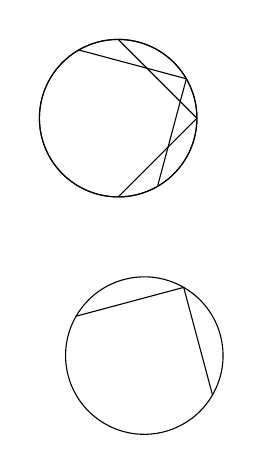
\begin{tikzpicture}

%\draw(0,0) circle (2);
%pump
\draw(0,0) circle (1);
\draw(1,0) -- (0,1);
\draw(1,0) -- (0,-1);

\begin{scope} [rotate=30]
    \draw[transform shape] (0,0) circle (1);
\draw[transform shape] (1,0) -- (0,1);
\draw[transform shape] (1,0) -- (0,-1);
  \end{scope}

\begin{scope} [rotate=60, shift={(-2.4451,-1.7951)}]
    \draw[transform shape] (0,0) circle (1);
\draw[transform shape] (1,0) -- (0,1);
\draw[transform shape] (1,0) -- (0,-1);
  \end{scope}


\end{tikzpicture}
\end{figure}